\section*{Sequential Implementation}
We first develop a sequential solution to the Wavefront problem in order to identify potential parallelization opportunities. The simplest approach is to compute the diagonals sequentially, starting from the first after the major diagonal and ending with the last. Each diagonal has one less element than the previous, and computation on the next diagonal begins only after completing the current one. A basic pseudocode is shown in Algorithm \ref{Algo1}.  

\begin{algorithm}
\begin{algorithmic}
% We assume the major diagonal has index 0, so we start at index 1
\FOR{diag = 1 \textbf{to} matrix\_length - 1}
    \FOR{elem = 1 \textbf{to} diag\_length}
        \STATE Compute(elem)
    \ENDFOR
\ENDFOR
\end{algorithmic}
\caption{Basic Wavefront Sequential Pattern}
\label{Algo1}
\end{algorithm}


\subsection*{The SquareMatrix class}
\par 
In all implementations, the square matrix is represented by the custom \texttt{SquareMatrix} class. The matrix data is stored internally in a \texttt{std::vector<double>} of size $n \times n$, where $n$ is the number of rows and columns. By using a single vector instead of a \texttt{std::vector<std::vector<double>>}, we optimize both storage and efficiency.

\par The class provides methods to store and retrieve elements using row and column indices, hiding the underlying implementation to the user. Given a matrix \texttt{mtx} of type \texttt{SquareMatrix}, then an element is indexed as follows:
\begin{equation}
    \forall i \in [0, n - 1]. \forall j \in [0, n - 1]. mtx[i][j] = data[(i * n) + j]
\end{equation}
By offering methods that avoid the need to explicitly write the above formula we prevent potential bugs caused by typos when applying it multiple times in the project.

\par Additionally, the class features the method \texttt{InitializeMatrix} which sets the values of the major diagonal according to the project's requirements.

\begin{figure}[h]
    \centering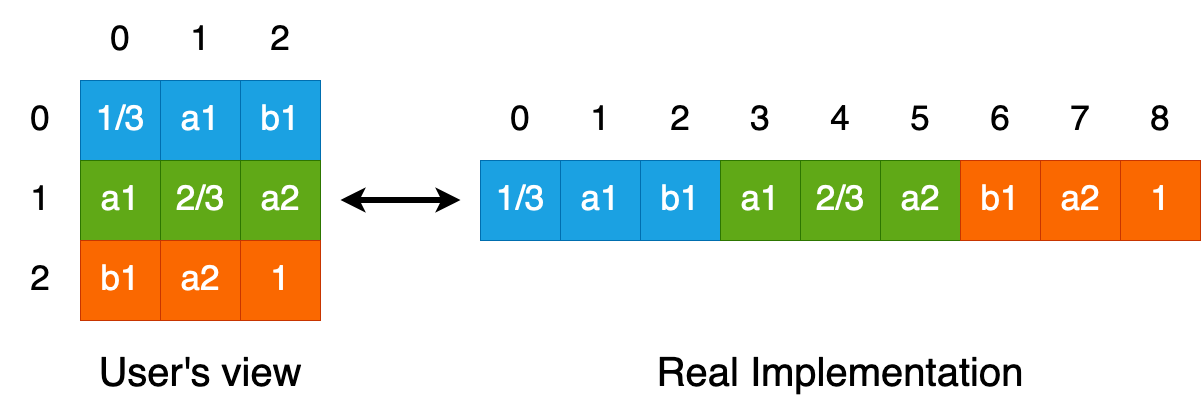
\includegraphics[scale=0.30]{img/Sequential Implementation/SquareMatriximpl.drawio.png}
    
    \caption{How the user sees a square matrix and its real implementation.}
\end{figure}

\subsection*{Cache Optimization}
When computing an element of an upper diagonal, we need to calculate the dot product of its associated row and column vectors. Since the matrix is stored in a single \texttt{std::vector<double>}, elements are stored contiguously by rows. As a result, when accessing a row vector, the processor can take advantage of the \textit{locality of reference} principle, storing adjacent elements in cache and optimizing retrieval during the dot product computation.
\par To achieve similar efficiency for column vectors, we can utilize the unused lower-triangular part of the matrix. Since all cells below the major diagonal are empty and unused in the Wavefront pattern, we can copy the values of the upper-triangular columns into the transposed rows of the lower-triangular part, such that:
\begin{equation}
    \forall i \in [0, n - 1]. \forall j \in [0, n - 1]. mtx[i][j] = mtx[j][i]
\end{equation}
By retrieving elements of the column vector in their corresponding lower-triangular row, we both utilize wasted space in the matrix and let the processor benefit from the \textit{locality of reference} principle for both vectors, making the dot product more efficient.

\par To facilitate this process, the \texttt{SquareMatrix} class provides the method \texttt{SetValue(row, col, val)}, which stores the value in both the original and transposed positions within the matrix.

\begin{figure}[h]
    \centering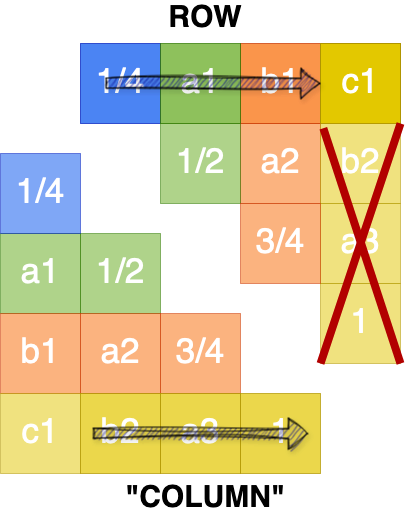
\includegraphics[scale=0.30]{img/Sequential Implementation/Locality_of_reference.drawio.png}
    
    \caption{Example of a dot product computation for the element \texttt{c1} in a 4x4 Matrix.}
\end{figure}

\subsection*{Asymptotic Complexity}
For an $n \times n$ matrix, the asymptotic complexity of a Wavefront computation is determined by the processing of all upper diagonals. The $i^{th}$ diagonal has a length of $n - i$, which is equal to the number of elements to compute. Each element of a diagonal requires a dot product between vectors of length $n - i - 1$ and the application of the cube root to the result. Assuming both the cost of multiplying two elements and applying the cube root is $\mathcal{O}(1)$, then:

\begin{itemize}
    \item \textbf{Complexity of computing an element of a diagonal = } $k \times \mathcal{O}(1) + \mathcal{O}(1) = \mathcal{O}(k)$ where $k$ is the length of the vectors. 

    \item \textbf{Complexity of computing all elements of one diagonal =} $z \times \mathcal{O}(z-1) = \mathcal{O}(z^{2})$ where $z$ is the length of the diagonal.

    \item \textbf{Overall complexity = } $n-1 \times \mathcal{O}((n-1)^{2}) = \mathcal{O}(n^{3})$ where $n$ is the length of the matrix.
\end{itemize}

\subsection*{Measurements}
A C++ implementation of the sequential approach stored in \textit{``src/sequential.cpp''} has been developed to study its time complexity compared to the more efficient parallel algorithms introduced in the following sections. All project code was tested on the \textit{"spmcluster.unipi.it"} compute cluster at the University of Pisa, using various matrix sizes. Each test was run five times per matrix size, and the graphs present the average results for each size.

\begin{figure}[h]
    \centering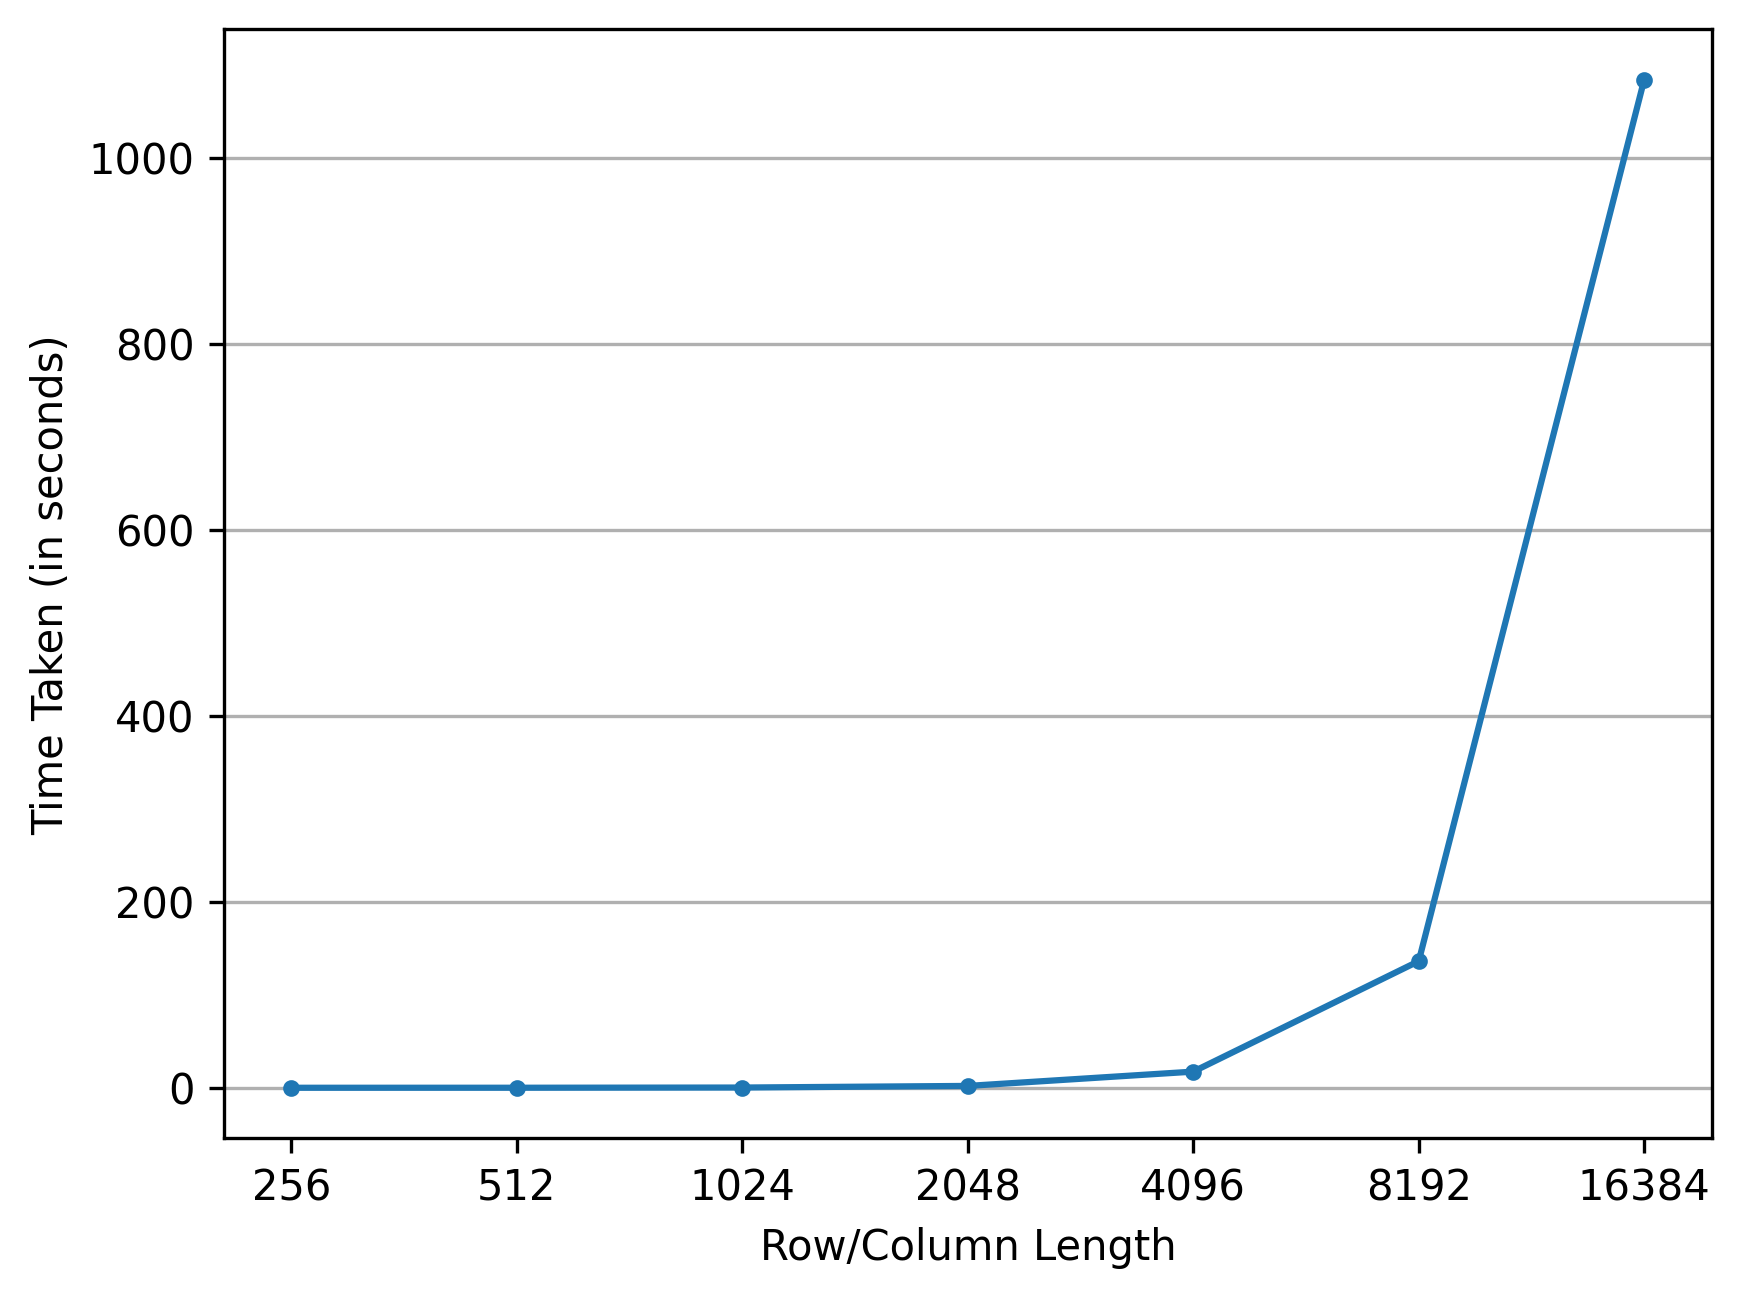
\includegraphics[scale=0.50]{img/Sequential Implementation/sequential_graph.png}
    \caption{Time measurements in seconds of the sequential implementation of the algorithm.}
\end{figure}

